
%(BEGIN_QUESTION)
% Copyright 2009, Tony R. Kuphaldt, released under the Creative Commons Attribution License (v 1.0)
% This means you may do almost anything with this work of mine, so long as you give me proper credit

Calculate the amount of differential pressure ``seen'' by this pneumatic DP transmitter across this baghouse (used to filter dust from air) in units of PSID and units of bar (differential), then calculate its output signal (in units of PSIG) assuming a calibrated range of 0 to 30 inches water column differential:

$$\includegraphics[width=15.5cm]{i03935x01.eps}$$

\vskip 20pt \vbox{\hrule \hbox{\strut \vrule{} {\bf Suggestions for Socratic discussion} \vrule} \hrule}

\begin{itemize}
\item{} Why do you suppose it is important to continuously measure the pressure differential across an industrial baghouse?
\item{} Why measure {\it differential} pressure across the baghouse, rather than simply measure either the upstream or downstream ({\it gauge}) pressure?
\item{} How would a rip in one of the fabric bags affect the differential pressure drop across the baghouse?
\item{} Suppose a technician accidently left one of the block valves shut on one of the transmitter's impulse lines.  How might this change affect the transmitter's ability to sense differential pressure?
\item{} Suppose a technician accidently left the equalizing valve open between the transmitter's impulse lines.  How might this change affect the transmitter's ability to sense differential pressure?
\end{itemize}

\underbar{file i03935}
%(END_QUESTION)





%(BEGIN_ANSWER)

\noindent
{\bf Partial answer:}

\vskip 10pt

Applied differential pressure = 0.969 PSID = 0.0668 bar (differential)

%(END_ANSWER)





%(BEGIN_NOTES)

$P_{high}$ = 0.498 kPa = 0.07223 PSIG

$P_{low}$ = 0.939 Atm = 13.8033 PSIA = $-0.8967$ PSIG

$\Delta P$ = 0.07223 PSIG $-$ ($-0.8967$ PSIG) = 0.9689 PSID

\vskip 10pt

Transmitter output signal = 13.73 PSI

\vskip 10pt

The air temperature shown in the illustration is extraneous information, included for the purpose of challenging students to identify whether or not information is relevant to solving a particular problem.

%INDEX% Physics, units and conversions: pressure
%INDEX% Process: baghouse filter (generic)

%(END_NOTES)


